\section{Übung 9 – Statistische Verteilungen und Momente}

In dieser Übung werden die wichtigsten Wahrscheinlichkeitsverteilungen aus
Kapitel~4 auf konkrete Aufgabenstellungen angewandt: die Poisson-Verteilung
(Abschnitt~\ref{sec:poisson-verteilung}) am Beispiel eines tropfenden Rohres,
die kontinuierliche und diskrete Gleichverteilung
(Abschnitt~\ref{sec:gleichverteilung}), die Normalverteilung
(Abschnitt~\ref{sec:normalverteilung}) im Rahmen eines Detektorproblems,
statistische Mittelwerte diskreter Zufallsvariablen sowie die Laplace-
(Abschnitt~\ref{sec:laplaceverteilung}) und die Exponentialverteilung
(Abschnitt~\ref{sec:exponentialverteilung}). Alle Aufgaben nutzen die
Definitionen von Erwartungswert (Abschnitt~\ref{sec:erwartungswert-kontinuierlich}),
Momenten und Varianz (Abschnitt~\ref{sec:momente}) sowie der
Verteilungsfunktion (Abschnitt~\ref{sec:verteilungsfunktion}).

% ================================================================
\subsection*{Vorrechenaufgabe 9 – Poisson-Verteilung (tropfendes Rohr)}
% ================================================================

Aus einem defekten Wasserrohr tropft es mit der mittleren Tropfrate
$\lambda = 5\,\mathrm{min}^{-1}$. Die Anzahl $k$ der in einem
Beobachtungsintervall der Länge $T_B$ gefallenen Tropfen ist Poisson-verteilt
gemäß

$$
P\bigl(X(T_B) = k\bigr) = C \cdot \frac{(\lambda T_B)^k}{k!}\, e^{-\lambda T_B},
\qquad k \in \{0, 1, 2, \dots\}.
$$

Jeder Tropfen besitzt ein Volumen von $0{,}05\,\mathrm{ml}$; der Eimer fasst
$1\,\mathrm{Liter} = 1000\,\mathrm{ml}$.

% ---- a) --------------------------------------------------------
\subsubsection*{a) Normierungskonstante $C$}

\begin{beispiel}[Normierung der Poisson-Verteilung]

\textbf{Gegeben:} Verteilung $P(X(T_B)=k) = C\,(\lambda T_B)^k/k!\; e^{-\lambda T_B}$.

\textbf{Gesucht:} Konstante $C$, so dass eine gültige Wahrscheinlichkeitsverteilung
vorliegt.

\textbf{Formel} (Normierungsbedingung sowie Reihe $e^{x} = \sum_{k=0}^{\infty} x^k/k!$):

$$
\sum_{k=0}^{\infty} P\bigl(X(T_B) = k\bigr) = 1
$$

\textbf{Rechnung:}

$$
\sum_{k=0}^{\infty} C\, \frac{(\lambda T_B)^k}{k!}\, e^{-\lambda T_B}
= C\, e^{-\lambda T_B} \sum_{k=0}^{\infty} \frac{(\lambda T_B)^k}{k!}
= C\, e^{-\lambda T_B}\, e^{\lambda T_B}
= C \;\overset{!}{=}\; 1.
$$

\textbf{Lösung:}

$$
\boxed{\;C = 1\;}
$$

Die angegebene Verteilung ist bereits die (normierte) Poisson-Verteilung mit
Parameter $\mu = \lambda T_B$; es ist kein zusätzlicher Faktor nötig.

\end{beispiel}

% ---- b) --------------------------------------------------------
\subsubsection*{b) Erwartungswert, zweites Moment, Varianz}

\begin{beispiel}[Momente der Poisson-Verteilung]

\textbf{Gegeben:} Poisson-Verteilung mit Parameter $\mu = \lambda T_B$.

\textbf{Gesucht:} $\mathrm{E}\{X\}$, $\mathrm{E}\{X^2\}$ und $\mathrm{var}\{X\}$.

\textbf{Formel} (Momente der Poisson-Verteilung, Abschnitt~\ref{sec:poisson-verteilung}):

$$
\mathrm{E}\{X\} = \mu, \qquad \mathrm{E}\{X^2\} = \mu^2 + \mu, \qquad
\mathrm{var}\{X\} = \mathrm{E}\{X^2\} - \mathrm{E}\{X\}^2 = \mu.
$$

\textbf{Rechnung:} Mit $\mu = \lambda T_B$ folgt unmittelbar

$$
\mathrm{E}\{X\} = \lambda T_B, \qquad
\mathrm{E}\{X^2\} = (\lambda T_B)^2 + \lambda T_B, \qquad
\mathrm{var}\{X\} = (\lambda T_B)^2 + \lambda T_B - (\lambda T_B)^2 = \lambda T_B.
$$

\textbf{Lösung:}

$$
\boxed{\;\mathrm{E}\{X\} = \lambda T_B, \qquad
\mathrm{E}\{X^2\} = (\lambda T_B)^2 + \lambda T_B, \qquad
\mathrm{var}\{X\} = \lambda T_B\;}
$$

Bei der Poisson-Verteilung stimmen Erwartungswert und Varianz überein
($\mathrm{E}\{X\} = \mathrm{var}\{X\} = \lambda T_B$).

\end{beispiel}

% ---- c) --------------------------------------------------------
\subsubsection*{c) Wahrscheinlichkeit für 20 Tropfen in 2 Minuten}

\begin{beispiel}[Poisson-Einzelwahrscheinlichkeit]

\textbf{Gegeben:} $\lambda = 5\,\mathrm{min}^{-1}$, $T_B = 2\,\mathrm{min}$,
also $\mu = \lambda T_B = 10$.

\textbf{Gesucht:} $P\bigl(X(T_B) = 20\bigr)$.

\textbf{Formel:}

$$
P\bigl(X(T_B) = k\bigr) = \frac{\mu^k}{k!}\, e^{-\mu}
$$

\textbf{Rechnung:}

$$
P\bigl(X = 20\bigr) = \frac{10^{20}}{20!}\, e^{-10}
= \frac{10^{20}}{2{,}4329 \cdot 10^{18}}\, \cdot 4{,}540 \cdot 10^{-5}
= 41{,}103 \cdot 4{,}540 \cdot 10^{-5}.
$$

\textbf{Lösung:}

$$
\boxed{\;P\bigl(X = 20\bigr) = \frac{10^{20}}{20!}\, e^{-10} \approx 1{,}87 \cdot 10^{-3}\;}
$$

Obwohl der Erwartungswert genau bei $\mu = 10$ liegt, ist die
Wahrscheinlichkeit für exakt $20$ Tropfen mit rund $0{,}19\,\%$ sehr klein --
das doppelte des Mittelwertes liegt weit in der Flanke der Verteilung.

\end{beispiel}

% ---- d) --------------------------------------------------------
\subsubsection*{d) Wahrscheinlichkeit für mindestens $0{,}25\,\mathrm{ml}$ in einer Minute}

\begin{beispiel}[Poisson-Summenwahrscheinlichkeit]

\textbf{Gegeben:} $\lambda = 5\,\mathrm{min}^{-1}$, $T_B = 1\,\mathrm{min}$,
also $\mu = 5$. Ein Tropfen hat $0{,}05\,\mathrm{ml}$; $0{,}25\,\mathrm{ml}$
entsprechen $0{,}25/0{,}05 = 5$ Tropfen.

\textbf{Gesucht:} $P(X \geq 5)$.

\textbf{Formel} (Gegenereignis):

$$
P(X \geq 5) = 1 - P(X \leq 4) = 1 - \sum_{k=0}^{4} \frac{\mu^k}{k!}\, e^{-\mu}
$$

\textbf{Rechnung:} Mit $e^{-5} = 6{,}7379 \cdot 10^{-3}$ und

$$
\sum_{k=0}^{4} \frac{5^k}{k!} = 1 + 5 + \frac{25}{2} + \frac{125}{6} + \frac{625}{24}
= 1 + 5 + 12{,}5 + 20{,}833 + 26{,}042 = 65{,}375
$$

folgt

$$
P(X \leq 4) = 65{,}375 \cdot 6{,}7379 \cdot 10^{-3} = 0{,}4405,
\qquad P(X \geq 5) = 1 - 0{,}4405.
$$

\textbf{Lösung:}

$$
\boxed{\;P(X \geq 5) = 1 - \sum_{k=0}^{4} \frac{5^k}{k!}\, e^{-5} \approx 0{,}5595\;}
$$

Mit rund $56\,\%$ ist es etwas wahrscheinlicher als nicht, dass in einer Minute
mindestens $0{,}25\,\mathrm{ml}$ zusammenkommen (Erwartung: $5$ Tropfen
$\hat{=}\, 0{,}25\,\mathrm{ml}$).

\end{beispiel}

% ---- e) --------------------------------------------------------
\subsubsection*{e) Kein Tropfen während der 30\,s Entleerung}

\begin{beispiel}[Wahrscheinlichkeit für kein Ereignis]

\textbf{Gegeben:} Entleerungsdauer $T_B = 30\,\mathrm{s} = 0{,}5\,\mathrm{min}$,
also $\mu = \lambda T_B = 5 \cdot 0{,}5 = 2{,}5$. Während dieser Zeit ist der
Eimer entfernt; ein fallender Tropfen träfe den Boden.

\textbf{Gesucht:} $P(X = 0)$ (kein Tropfen auf den Boden).

\textbf{Formel:}

$$
P(X = 0) = \frac{\mu^0}{0!}\, e^{-\mu} = e^{-\mu}
$$

\textbf{Rechnung:}

$$
P(X = 0) = e^{-2{,}5} = 0{,}0821.
$$

\textbf{Lösung:}

$$
\boxed{\;P(X = 0) = e^{-2{,}5} \approx 0{,}0821\;}
$$

Nur in rund $8{,}2\,\%$ der Entleerungen bleibt der Boden trocken -- meist fällt
in den $30\,\mathrm{s}$ mindestens ein Tropfen daneben.

\end{beispiel}

% ---- f) --------------------------------------------------------
\subsubsection*{f) Boden genau fünfmal nass in einer Woche}

\begin{beispiel}[Verkettung von Poisson und Binomialverteilung]

\textbf{Gegeben:} Der Eimer wird einmal täglich entleert (Dauer $30\,\mathrm{s}$).
Aus Teil~e) ist die Wahrscheinlichkeit, dass der Boden bei \emph{einer}
Entleerung nass wird,

$$
p = P(\text{Boden nass}) = 1 - P(X = 0) = 1 - e^{-2{,}5} = 0{,}9179.
$$

Eine Woche umfasst $n = 7$ unabhängige Entleerungen.

\textbf{Gesucht:} $P(\text{genau } 5\text{-mal nass in } 7 \text{ Tagen})$.

\textbf{Formel} (Binomialverteilung, Abschnitt~\ref{sec:binomialverteilung}):

$$
P(K = k) = \binom{n}{k}\, p^k\, (1 - p)^{n - k}
$$

\textbf{Rechnung:} Mit $n = 7$, $k = 5$, $p = 0{,}9179$, $1 - p = 0{,}0821$:

$$
P(K = 5) = \binom{7}{5}\, (0{,}9179)^5\, (0{,}0821)^2
= 21 \cdot 0{,}6517 \cdot 0{,}006738.
$$

\textbf{Lösung:}

$$
\boxed{\;P(K = 5) = \binom{7}{5}\,\bigl(1 - e^{-2{,}5}\bigr)^5\,\bigl(e^{-2{,}5}\bigr)^2
\approx 0{,}0922\;}
$$

Da der Boden pro Tag mit über $91\,\%$ nass wird, ist \emph{genau} fünf nasse
Tage (statt sechs oder sieben) eher unwahrscheinlich -- $P(K=7) \approx 0{,}55$
und $P(K=6) \approx 0{,}34$ dominieren.

\end{beispiel}

% ================================================================
\subsection*{Aufgabe 9.1 – Gleichverteilung auf $[-1, 2]$}
% ================================================================

Die kontinuierliche Zufallsvariable $X$ ist auf dem Intervall $[a, b] = [-1, 2]$
gleichverteilt (Abschnitt~\ref{sec:gleichverteilung}), also mit
$b - a = 3$:

$$
p_X(x) = \begin{cases} \dfrac{1}{3} & , \quad -1 \leq x \leq 2 \\[6pt]
0 & , \quad \text{sonst.} \end{cases}
$$

% ---- a) --------------------------------------------------------
\subsubsection*{a) Kumulative Verteilungsfunktion}

\begin{beispiel}[Verteilungsfunktion der Gleichverteilung]

\textbf{Gegeben:} $p_X(x) = 1/3$ für $-1 \leq x \leq 2$ (sonst $0$).

\textbf{Gesucht:} Die kumulative Verteilungsfunktion $F_X(x)$ und ihre grafische
Darstellung.

\textbf{Formel} (Abschnitt~\ref{sec:verteilungsfunktion}):

$$
F_X(x) = \int_{-\infty}^{x} p_X(u)\,\mathrm{d}u
$$

\textbf{Rechnung:} Für $-1 \leq x \leq 2$ gilt

$$
F_X(x) = \int_{-1}^{x} \frac{1}{3}\,\mathrm{d}u = \frac{x - (-1)}{3} = \frac{x + 1}{3}.
$$

Für $x < -1$ ist $F_X(x) = 0$, für $x > 2$ ist $F_X(x) = 1$.

\textbf{Lösung:}

$$
\boxed{\;F_X(x) = \begin{cases}
0 & , \quad x < -1 \\[4pt]
\dfrac{x + 1}{3} & , \quad -1 \leq x \leq 2 \\[8pt]
1 & , \quad x > 2 \end{cases}\;}
$$

\begin{center}
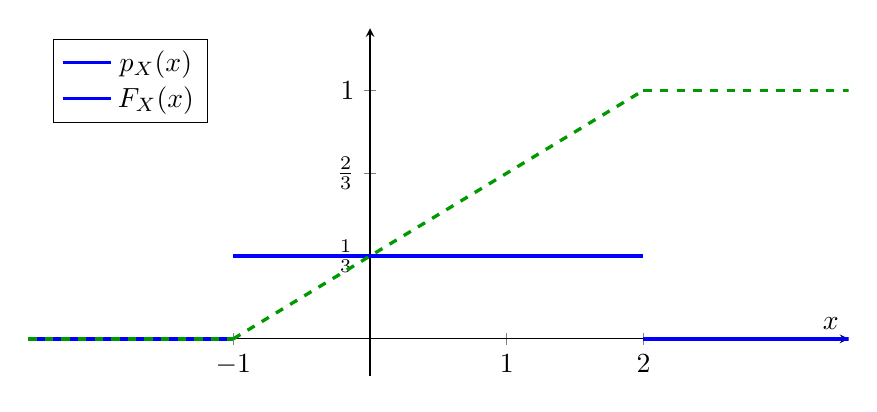
\begin{tikzpicture}
\begin{axis}[
  width=12cm, height=6cm,
  xmin=-2.5, xmax=3.5, ymin=-0.15, ymax=1.25,
  axis lines=center, xlabel={$x$},
  xtick={-1,0,1,2}, ytick={0.3333,0.6667,1},
  yticklabels={$\frac13$,$\frac23$,$1$},
  legend pos=north west,
  every axis plot/.append style={very thick},
]
\addplot[blue] coordinates {(-2.5,0) (-1,0)};
\addplot[blue] coordinates {(-1,0.3333) (2,0.3333)};
\addplot[blue] coordinates {(2,0) (3.5,0)};
\addlegendentry{$p_X(x)$}
\addplot[green!60!black, dashed] coordinates {(-2.5,0) (-1,0)};
\addplot[green!60!black, dashed] coordinates {(-1,0) (2,1)};
\addplot[green!60!black, dashed] coordinates {(2,1) (3.5,1)};
\addlegendentry{$F_X(x)$}
\end{axis}
\end{tikzpicture}
\end{center}

\end{beispiel}

% ---- b) --------------------------------------------------------
\subsubsection*{b) Erwartungswert, zweites Moment, Varianz}

\begin{beispiel}[Momente der Gleichverteilung]

\textbf{Gegeben:} Gleichverteilung auf $[a, b] = [-1, 2]$.

\textbf{Gesucht:} $\mathrm{E}\{X\}$, $\mathrm{E}\{X^2\}$, $\mathrm{var}\{X\}$.

\textbf{Formel} (Abschnitt~\ref{sec:gleichverteilung}):

$$
\mathrm{E}\{X\} = \frac{a + b}{2}, \qquad
\mathrm{E}\{X^2\} = \frac{a^2 + ab + b^2}{3}, \qquad
\mathrm{var}\{X\} = \frac{(a - b)^2}{12}.
$$

\textbf{Rechnung:} Mit $a = -1$, $b = 2$:

$$
\mathrm{E}\{X\} = \frac{-1 + 2}{2} = \frac{1}{2}, \qquad
\mathrm{E}\{X^2\} = \frac{1 - 2 + 4}{3} = \frac{3}{3} = 1,
$$
$$
\mathrm{var}\{X\} = \frac{(-1 - 2)^2}{12} = \frac{9}{12} = \frac{3}{4}.
$$

Kontrolle: $\mathrm{var}\{X\} = \mathrm{E}\{X^2\} - \mathrm{E}\{X\}^2
= 1 - \tfrac{1}{4} = \tfrac{3}{4}$. \checkmark

\textbf{Lösung:}

$$
\boxed{\;\mathrm{E}\{X\} = \frac{1}{2} = 0{,}5, \qquad
\mathrm{E}\{X^2\} = 1, \qquad
\mathrm{var}\{X\} = \frac{3}{4} = 0{,}75\;}
$$

\end{beispiel}

% ---- c) --------------------------------------------------------
\subsubsection*{c) $P(X \in [-1, 1])$}

\begin{beispiel}[Intervallwahrscheinlichkeit der Gleichverteilung]

\textbf{Gegeben:} $p_X(x) = 1/3$ auf $[-1, 2]$.

\textbf{Gesucht:} $P(-1 \leq X \leq 1)$.

\textbf{Formel:}

$$
P(X \in [c, d]) = \int_c^d p_X(u)\,\mathrm{d}u = F_X(d) - F_X(c)
$$

\textbf{Rechnung:}

$$
P(-1 \leq X \leq 1) = \int_{-1}^{1} \frac{1}{3}\,\mathrm{d}u
= \frac{1 - (-1)}{3} = \frac{2}{3}.
$$

\textbf{Lösung:}

$$
\boxed{\;P(-1 \leq X \leq 1) = \frac{2}{3} \approx 0{,}667\;}
$$

\end{beispiel}

% ---- d) --------------------------------------------------------
\subsubsection*{d) $P(X \geq 0)$}

\begin{beispiel}[Halbseitige Wahrscheinlichkeit]

\textbf{Gegeben:} $p_X(x) = 1/3$ auf $[-1, 2]$.

\textbf{Gesucht:} $P(X \geq 0)$.

\textbf{Formel:}

$$
P(X \geq 0) = \int_0^{2} p_X(u)\,\mathrm{d}u = 1 - F_X(0)
$$

\textbf{Rechnung:}

$$
P(X \geq 0) = \int_0^{2} \frac{1}{3}\,\mathrm{d}u = \frac{2 - 0}{3} = \frac{2}{3}.
$$

\textbf{Lösung:}

$$
\boxed{\;P(X \geq 0) = \frac{2}{3} \approx 0{,}667\;}
$$

\end{beispiel}

% ---- e) --------------------------------------------------------
\subsubsection*{e) $P(X \in [a, b])$ für $b - a \to 0$}

\begin{beispiel}[Wahrscheinlichkeit eines infinitesimalen Intervalls]

\textbf{Gegeben:} Ein Intervall $[\alpha, \beta] \subseteq [-1, 2]$ mit
Länge $\beta - \alpha \to 0$.

\textbf{Gesucht:} Der Grenzwert von $P(\alpha \leq X \leq \beta)$.

\textbf{Formel:}

$$
P(\alpha \leq X \leq \beta) = \int_{\alpha}^{\beta} \frac{1}{3}\,\mathrm{d}u
= \frac{\beta - \alpha}{3}
$$

\textbf{Rechnung:}

$$
\lim_{\beta - \alpha \to 0} P(\alpha \leq X \leq \beta)
= \lim_{\beta - \alpha \to 0} \frac{\beta - \alpha}{3} = 0.
$$

\textbf{Lösung:}

$$
\boxed{\;P(\alpha \leq X \leq \beta) \xrightarrow{\;\beta - \alpha \to 0\;} 0
\quad\Longrightarrow\quad P(X = x_0) = 0\;}
$$

Bei einer kontinuierlichen Zufallsvariablen besitzt jeder \emph{einzelne} Wert
die Wahrscheinlichkeit $0$; nur Intervalle positiver Länge tragen
Wahrscheinlichkeitsmasse.

\end{beispiel}

% ---- f) --------------------------------------------------------
\subsubsection*{f) Diskrete Gleichverteilung auf $\{-1, 0, 1, 2\}$}

\begin{beispiel}[Diskrete Gleichverteilung -- PMF und CDF]

\textbf{Gegeben:} Nur die ganzzahligen Werte $x_i \in \{-1, 0, 1, 2\}$ sind
zulässig, jeder mit gleicher Wahrscheinlichkeit.

\textbf{Gesucht:} Die Wahrscheinlichkeitsverteilung $P(X = x_i)$ und die
kumulative Verteilungsfunktion $F_X(x)$ nebst Darstellung.

\textbf{Formel} (diskrete Gleichverteilung über $M$ Werten):

$$
P(X = x_i) = \frac{1}{M}, \qquad F_X(x) = \sum_{x_i \leq x} P(X = x_i)
$$

\textbf{Rechnung:} Es gibt $M = 4$ gleichwahrscheinliche Werte:

$$
P(X = x_i) = \frac{1}{4} \quad \text{für } x_i \in \{-1, 0, 1, 2\}.
$$

Die kumulative Verteilung springt an jedem $x_i$ um $\tfrac14$:

$$
F_X(x) = \begin{cases}
0 & , \quad x < -1 \\
\tfrac{1}{4} & , \quad -1 \leq x < 0 \\
\tfrac{2}{4} & , \quad 0 \leq x < 1 \\
\tfrac{3}{4} & , \quad 1 \leq x < 2 \\
1 & , \quad x \geq 2.
\end{cases}
$$

\textbf{Lösung:}

$$
\boxed{\;P(X = x_i) = \frac{1}{4}\ \text{für } x_i \in \{-1,0,1,2\}; \qquad
F_X(x)\ \text{Treppenfunktion mit Sprüngen } \tfrac14\;}
$$

\begin{center}
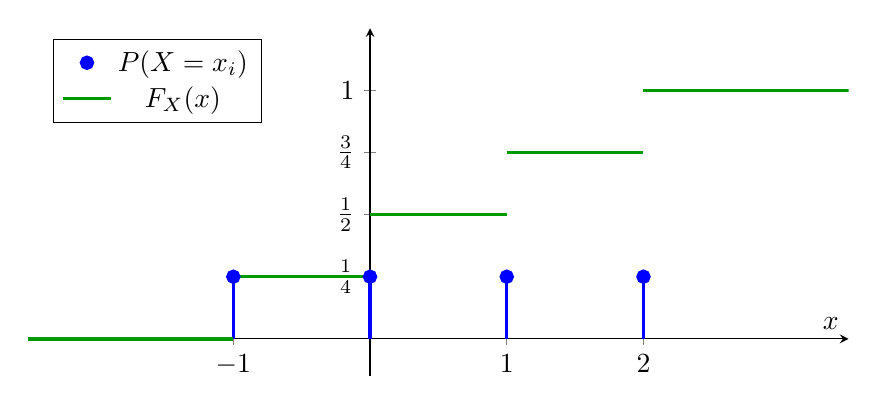
\begin{tikzpicture}
\begin{axis}[
  width=12cm, height=6cm,
  xmin=-2.5, xmax=3.5, ymin=-0.15, ymax=1.25,
  axis lines=center, xlabel={$x$},
  xtick={-1,0,1,2}, ytick={0.25,0.5,0.75,1},
  yticklabels={$\frac14$,$\frac12$,$\frac34$,$1$},
  legend pos=north west,
]
% PMF als Stem-Plot
\addplot[blue, ycomb, mark=*, very thick] coordinates {(-1,0.25) (0,0.25) (1,0.25) (2,0.25)};
\addlegendentry{$P(X = x_i)$}
% CDF als Treppenfunktion
\addplot[green!60!black, very thick] coordinates {(-2.5,0) (-1,0)};
\addplot[green!60!black, very thick] coordinates {(-1,0.25) (0,0.25)};
\addplot[green!60!black, very thick] coordinates {(0,0.5) (1,0.5)};
\addplot[green!60!black, very thick] coordinates {(1,0.75) (2,0.75)};
\addplot[green!60!black, very thick] coordinates {(2,1) (3.5,1)};
\addlegendentry{$F_X(x)$}
\end{axis}
\end{tikzpicture}
\end{center}

\end{beispiel}

% ---- g) --------------------------------------------------------
\subsubsection*{g) Diskrete Fassung von d), e) sowie $P(X = 1)$}

\begin{beispiel}[Diskret vs.\ kontinuierlich -- der Unterschied am einzelnen Punkt]

\textbf{Gegeben:} Diskrete Gleichverteilung auf $\{-1, 0, 1, 2\}$ mit
$P(X = x_i) = \tfrac14$.

\textbf{Gesucht:} $P(X \geq 0)$ (Teil d), $P(X = x_0)$ für einen einzelnen Wert
(Teil e) sowie $P(X = 1)$; Vergleich mit dem kontinuierlichen Fall.

\textbf{Formel:}

$$
P(X \in A) = \sum_{x_i \in A} P(X = x_i)
$$

\textbf{Rechnung:}

\emph{Zu d):} Die Werte $\geq 0$ sind $\{0, 1, 2\}$, also

$$
P(X \geq 0) = P(0) + P(1) + P(2) = \frac{3}{4}.
$$

\emph{Zu e):} Ein einzelner zulässiger Wert hat nun \emph{positive}
Wahrscheinlichkeit; das Intervall lässt sich nicht mehr beliebig verkleinern,
ohne einen Massepunkt zu treffen:

$$
P(X = x_0) = \frac{1}{4} \neq 0.
$$

\emph{Speziell:} $\displaystyle P(X = 1) = \frac{1}{4}$.

\textbf{Lösung:}

$$
\boxed{\;P(X \geq 0) = \frac{3}{4}, \qquad P(X = x_0) = \frac{1}{4}, \qquad
P(X = 1) = \frac{1}{4}\;}
$$

\textbf{Unterschied zur kontinuierlichen Verteilung:} Im kontinuierlichen Fall
ist $P(X = 1) = 0$ (Teil~e), da die Wahrscheinlichkeitsmasse „verschmiert`` über
das Intervall verteilt ist. Im diskreten Fall konzentriert sie sich in
$M = 4$ Punkten, so dass jeder Wert die endliche Wahrscheinlichkeit $\tfrac14$
trägt. Auch $P(X \geq 0)$ ändert sich von $\tfrac23$ (kontinuierlich) auf
$\tfrac34$ (diskret): Der diskrete Fall zählt den Randpunkt $x = 0$ als vollen
Massepunkt mit, während er kontinuierlich nur eine Nullmenge bildet.

\end{beispiel}

% ================================================================
\subsection*{Aufgabe 9.2 – Normalverteilung (binärer Detektor)}
% ================================================================

Ein Sensor liefert Information über eine binäre Zustandsvariable
$Z \in \{0, 1\}$ mit gleichwahrscheinlichen Realisierungen
($P(Z = 0) = P(Z = 1) = \tfrac12$). Die Messwerte $x = z + w$ sind durch
additives, normalverteiltes Rauschen $w$ und systematische Fehler gestört. Für
jeden Zustand liegen $N = 5$ Messwerte vor:

$$
z = 0:\ \{-1{,}9,\ 0{,}3,\ -0{,}8,\ 0{,}9,\ 0{,}4\}, \qquad
z = 1:\ \{1{,}8,\ -0{,}5,\ 2{,}0,\ -0{,}1,\ 0{,}4\}.
$$

% ---- a) --------------------------------------------------------
\subsubsection*{a) Schätzung von Mittelwert und Varianz}

\begin{beispiel}[Empirische Schätzung von Mittelwert und Varianz]

\textbf{Gegeben:} Je $N = 5$ Messwerte für $z = 0$ und $z = 1$.

\textbf{Gesucht:} $\mu_0, \mu_1$ und $\sigma_0^2, \sigma_1^2$.

\textbf{Formel} (empirischer Mittelwert und empirische Varianz,
Maximum-Likelihood-Schätzer mit Division durch $N$):

$$
\hat{\mu} = \frac{1}{N} \sum_{i=0}^{N-1} z_i, \qquad
\hat{\sigma}^2 = \frac{1}{N} \sum_{i=0}^{N-1} (z_i - \hat{\mu})^2
$$

\textbf{Rechnung:}

\emph{Zustand $z = 0$:}

$$
\mu_0 = \frac{-1{,}9 + 0{,}3 - 0{,}8 + 0{,}9 + 0{,}4}{5} = \frac{-1{,}1}{5} = -0{,}22.
$$

$$
\sum_i (z_i - \mu_0)^2 = 2{,}8224 + 0{,}2704 + 0{,}3364 + 1{,}2544 + 0{,}3844
= 5{,}068,
\qquad \sigma_0^2 = \frac{5{,}068}{5} = 1{,}0136.
$$

\emph{Zustand $z = 1$:}

$$
\mu_1 = \frac{1{,}8 - 0{,}5 + 2{,}0 - 0{,}1 + 0{,}4}{5} = \frac{3{,}6}{5} = 0{,}72.
$$

$$
\sum_i (z_i - \mu_1)^2 = 1{,}1664 + 1{,}4884 + 1{,}6384 + 0{,}6724 + 0{,}1024
= 5{,}068,
\qquad \sigma_1^2 = \frac{5{,}068}{5} = 1{,}0136.
$$

\textbf{Lösung:}

$$
\boxed{\;\mu_0 = -0{,}22, \quad \sigma_0^2 = 1{,}0136; \qquad
\mu_1 = 0{,}72, \quad \sigma_1^2 = 1{,}0136\;}
$$

Beide Stichproben besitzen (zufällig) dieselbe Varianz
$\sigma_0^2 = \sigma_1^2 = \sigma^2 = 1{,}0136$, also
$\sigma \approx 1{,}007$. Das vereinfacht die folgende Schwellwertbestimmung.

\end{beispiel}

% ---- b) --------------------------------------------------------
\subsubsection*{b) Parametrische Gaußsche Dichtemodelle}

\begin{beispiel}[Gaußsche Verteilungsdichtemodelle der beiden Zustände]

\textbf{Gegeben:} Geschätzte Parameter aus a).

\textbf{Gesucht:} Dichtemodelle $p_{Z,0}(z)$ und $p_{Z,1}(z)$.

\textbf{Formel} (Normalverteilung, Abschnitt~\ref{sec:normalverteilung}):

$$
p_{Z,k}(z) = \mathcal{N}(z;\, \mu_k,\, \sigma_k^2)
= \frac{1}{\sqrt{2\pi}\,\sigma_k}\, e^{-\frac{(z - \mu_k)^2}{2\sigma_k^2}}
$$

\textbf{Rechnung / Lösung:} Einsetzen der geschätzten Parameter:

$$
\boxed{\;
p_{Z,0}(z) = \frac{1}{\sqrt{2\pi \cdot 1{,}0136}}\,
e^{-\frac{(z + 0{,}22)^2}{2 \cdot 1{,}0136}}, \qquad
p_{Z,1}(z) = \frac{1}{\sqrt{2\pi \cdot 1{,}0136}}\,
e^{-\frac{(z - 0{,}72)^2}{2 \cdot 1{,}0136}}\;}
$$

\begin{center}
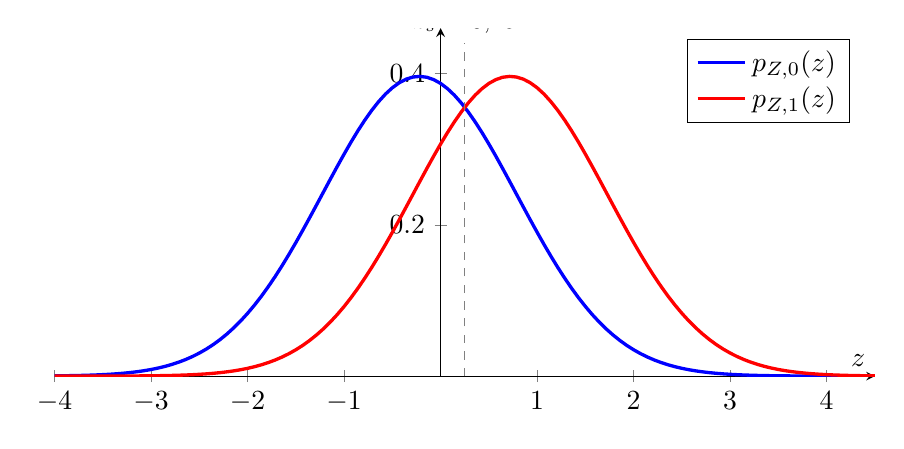
\begin{tikzpicture}
\begin{axis}[
  width=12cm, height=6cm,
  xmin=-4, xmax=4.5, ymin=0, ymax=0.46,
  axis lines=center, xlabel={$z$}, ylabel={},
  legend pos=north east,
  every axis plot/.append style={very thick},
  samples=120, domain=-4:4.5,
]
\addplot[blue] {1/sqrt(2*pi*1.0136)*exp(-(x+0.22)^2/(2*1.0136))};
\addlegendentry{$p_{Z,0}(z)$}
\addplot[red] {1/sqrt(2*pi*1.0136)*exp(-(x-0.72)^2/(2*1.0136))};
\addlegendentry{$p_{Z,1}(z)$}
\draw[dashed, gray] (axis cs:0.25,0) -- (axis cs:0.25,0.44);
\node[anchor=south, font=\small] at (axis cs:0.25,0.44) {$z_s = 0{,}25$};
\end{axis}
\end{tikzpicture}
\end{center}

\end{beispiel}

% ---- c) --------------------------------------------------------
\subsubsection*{c) Optimaler Schwellwert $z_s$}

\begin{beispiel}[Schwellwert minimaler Fehlerwahrscheinlichkeit]

\textbf{Gegeben:} Dichtemodelle aus b) mit gleichen Varianzen
$\sigma_0^2 = \sigma_1^2 = \sigma^2$ und gleichen a-priori-Wahrscheinlichkeiten
$P(Z=0) = P(Z=1) = \tfrac12$.

\textbf{Gesucht:} Schwellwert $z_s$ mit minimaler Fehlerwahrscheinlichkeit.

\textbf{Formel:} Der optimale Schwellwert liegt im Schnittpunkt der beiden
(gleich gewichteten) Dichten:

$$
p_{Z,0}(z_s) = p_{Z,1}(z_s)
$$

\textbf{Rechnung:} Bei gleicher Varianz $\sigma$ folgt aus der Gleichsetzung der
Exponenten

$$
(z_s - \mu_0)^2 = (z_s - \mu_1)^2
\quad\Longrightarrow\quad
z_s = \frac{\mu_0 + \mu_1}{2}
= \frac{-0{,}22 + 0{,}72}{2} = \frac{0{,}5}{2}.
$$

\textbf{Lösung:}

$$
\boxed{\;z_s = \frac{\mu_0 + \mu_1}{2} = 0{,}25\;}
$$

Da beide Zustände gleichwahrscheinlich sind und dieselbe Streuung besitzen,
liegt die optimale Entscheidungsgrenze genau mittig zwischen den beiden
Mittelwerten. Entscheidungsregel: $z < z_s \Rightarrow \hat{Z} = 0$,
$z \geq z_s \Rightarrow \hat{Z} = 1$.

\end{beispiel}

% ---- d) --------------------------------------------------------
\subsubsection*{d) Minimale Fehlerwahrscheinlichkeit $P_{e,\min}$}

\begin{beispiel}[Fehlerwahrscheinlichkeit des Gauß-Detektors]

\textbf{Gegeben:} $z_s = 0{,}25$, $\mu_0 = -0{,}22$, $\mu_1 = 0{,}72$,
$\sigma \approx 1{,}007$, gleiche a-priori-Wahrscheinlichkeiten.

\textbf{Gesucht:} $P_{e,\min}$.

\textbf{Formel} (Standardnormalverteilung $F_Y$ mit $Y = \tfrac{Z - \mu}{\sigma}$,
vgl.\ Hinweis und Abschnitt~\ref{sec:normalverteilung}):

$$
P_{e} = \tfrac{1}{2}\, P(Z > z_s \mid Z{=}0)
      + \tfrac{1}{2}\, P(Z < z_s \mid Z{=}1),
\qquad
F_Y(y) = \tfrac{1}{2}\!\left[1 + \operatorname{erf}\!\left(\tfrac{y}{\sqrt{2}}\right)\right].
$$

\textbf{Rechnung:} Wegen der Symmetrie ($z_s$ mittig, gleiche $\sigma$) sind
beide Fehlerterme gleich groß. Der standardisierte Abstand vom Schwellwert zu
jedem Mittelwert beträgt

$$
d = \frac{\mu_1 - z_s}{\sigma} = \frac{z_s - \mu_0}{\sigma}
= \frac{\mu_1 - \mu_0}{2\sigma}
= \frac{0{,}94}{2 \cdot 1{,}007} = 0{,}4668.
$$

Damit

$$
P_{e,\min} = 1 - F_Y(0{,}4668)
= \tfrac{1}{2}\!\left[1 - \operatorname{erf}\!\left(\tfrac{0{,}4668}{\sqrt{2}}\right)\right]
= \tfrac{1}{2}\!\left[1 - \operatorname{erf}(0{,}3301)\right]
= \tfrac{1}{2}\,(1 - 0{,}3599).
$$

\textbf{Lösung:}

$$
\boxed{\;P_{e,\min}
= \tfrac{1}{2}\operatorname{erfc}\!\left(\frac{\mu_1 - \mu_0}{2\sigma\sqrt{2}}\right)
= \tfrac{1}{2}\bigl[1 - \operatorname{erf}(0{,}3301)\bigr] \approx 0{,}320\;}
$$

Die minimale Fehlerwahrscheinlichkeit liegt bei rund $32\,\%$. Der Grund ist der
kleine Abstand der Mittelwerte im Verhältnis zur Streuung
($|\mu_1 - \mu_0|/\sigma \approx 0{,}93$): Die beiden Dichten überlappen stark,
so dass selbst der optimale Detektor häufig falsch entscheidet.

\end{beispiel}

% ================================================================
\subsection*{Aufgabe 9.3 – Statistische Mittelwerte}
% ================================================================

% ---- a) --------------------------------------------------------
\subsubsection*{a) Erwarteter Notendurchschnitt}

\begin{beispiel}[Erwartungswert, Varianz und Standardabweichung diskreter Noten]

\textbf{Gegeben:} Noten $w_i \in \{1, 2, 3, 4, 5\}$ mit den Wahrscheinlichkeiten

$$
P(w_i) = \{0{,}08,\ 0{,}28,\ 0{,}34,\ 0{,}22,\ 0{,}08\}.
$$

\textbf{Gesucht:} Erwartungswert $\mathrm{E}\{W\}$, Varianz $\mathrm{var}\{W\}$
und Standardabweichung $\sigma_W$.

\textbf{Formel} (diskreter Erwartungswert, Abschnitt~\ref{sec:erwartungswert}):

$$
\mathrm{E}\{W\} = \sum_i w_i\, P(w_i), \qquad
\mathrm{var}\{W\} = \mathrm{E}\{W^2\} - \mathrm{E}\{W\}^2, \qquad
\sigma_W = \sqrt{\mathrm{var}\{W\}}.
$$

\textbf{Rechnung:}

$$
\mathrm{E}\{W\} = 1(0{,}08) + 2(0{,}28) + 3(0{,}34) + 4(0{,}22) + 5(0{,}08)
= 0{,}08 + 0{,}56 + 1{,}02 + 0{,}88 + 0{,}40 = 2{,}94.
$$

$$
\mathrm{E}\{W^2\} = 1(0{,}08) + 4(0{,}28) + 9(0{,}34) + 16(0{,}22) + 25(0{,}08)
= 0{,}08 + 1{,}12 + 3{,}06 + 3{,}52 + 2{,}00 = 9{,}78.
$$

$$
\mathrm{var}\{W\} = 9{,}78 - 2{,}94^2 = 9{,}78 - 8{,}6436 = 1{,}1364,
\qquad \sigma_W = \sqrt{1{,}1364} = 1{,}066.
$$

\textbf{Lösung:}

$$
\boxed{\;\mathrm{E}\{W\} = 2{,}94, \qquad
\mathrm{var}\{W\} = 1{,}1364, \qquad
\sigma_W \approx 1{,}066\;}
$$

Der erwartete Notendurchschnitt beträgt $2{,}94$ bei einer Streuung von rund
einer Notenstufe.

\end{beispiel}

% ---- b) --------------------------------------------------------
\subsubsection*{b) Optimaler Repräsentant der Quantisierungsstufen}

\begin{beispiel}[Minimierung des mittleren quadratischen Fehlers]

\textbf{Gegeben:} Quantisierungsstufen
$\hat{x}_i \in \{0{,}125,\ 0{,}375,\ 0{,}625,\ 0{,}875\}$ mit
$P(\hat{x}_i) = \{0{,}4,\ 0{,}3,\ 0{,}2,\ 0{,}1\}$.

\textbf{Gesucht:} Der Wert $\bar{\bar{x}}$, der den mittleren quadratischen
Fehler $\mathfrak{F} = \sum_i (\bar{\bar{x}} - \hat{x}_i)^2 P(\hat{x}_i)$
minimiert, sowie der minimale Fehler $\mathfrak{F}$.

\textbf{Formel:} $\mathfrak{F}(\bar{\bar{x}})$ wird durch Ableiten nach
$\bar{\bar{x}}$ und Nullsetzen minimiert. Man erhält den Erwartungswert:

$$
\frac{\mathrm{d}\mathfrak{F}}{\mathrm{d}\bar{\bar{x}}}
= \sum_i 2(\bar{\bar{x}} - \hat{x}_i) P(\hat{x}_i) \overset{!}{=} 0
\quad\Longrightarrow\quad
\bar{\bar{x}} = \sum_i \hat{x}_i\, P(\hat{x}_i) = \mathrm{E}\{\hat{X}\}.
$$

Der zugehörige minimale Fehler ist dann die Varianz
$\mathfrak{F} = \mathrm{E}\{\hat{X}^2\} - \bar{\bar{x}}^2 = \mathrm{var}\{\hat{X}\}$.

\textbf{Rechnung:}

$$
\bar{\bar{x}} = 0{,}125(0{,}4) + 0{,}375(0{,}3) + 0{,}625(0{,}2) + 0{,}875(0{,}1)
= 0{,}05 + 0{,}1125 + 0{,}125 + 0{,}0875 = 0{,}375.
$$

$$
\mathfrak{F} = \sum_i (\bar{\bar{x}} - \hat{x}_i)^2 P(\hat{x}_i)
= (0{,}25)^2 (0{,}4) + 0 + (0{,}25)^2 (0{,}2) + (0{,}5)^2 (0{,}1)
$$
$$
= 0{,}025 + 0 + 0{,}0125 + 0{,}025 = 0{,}0625.
$$

\textbf{Lösung:}

$$
\boxed{\;\bar{\bar{x}} = \mathrm{E}\{\hat{X}\} = 0{,}375, \qquad
\mathfrak{F}_{\min} = \mathrm{var}\{\hat{X}\} = 0{,}0625 = \frac{1}{16}\;}
$$

Der optimale Ersatzwert ist der Erwartungswert der Quantisierungsstufen; der
minimale mittlere quadratische Fehler entspricht genau ihrer Varianz.

\end{beispiel}

% ================================================================
\subsection*{Aufgabe 9.4 – Laplace-Verteilung}
% ================================================================

Gegeben ist die Funktion

$$
p_Y(y) = \frac{A}{2\sigma}\, e^{-\frac{|y|}{\sigma}},
$$

d.\,h.\ eine um $\mu = 0$ zentrierte Laplace-Verteilung
(Abschnitt~\ref{sec:laplaceverteilung}) mit Parameter $\sigma > 0$.

% ---- a) --------------------------------------------------------
\subsubsection*{a) Normierungskonstante $A$}

\begin{beispiel}[Normierung der Laplace-Dichte]

\textbf{Gegeben:} $p_Y(y) = \tfrac{A}{2\sigma}\, e^{-|y|/\sigma}$.

\textbf{Gesucht:} $A$, so dass eine gültige Wahrscheinlichkeitsdichte vorliegt.

\textbf{Formel} (Normierung, Abschnitt~\ref{sec:ws-dichte-eigenschaften}):

$$
\int_{-\infty}^{\infty} p_Y(y)\,\mathrm{d}y = 1
$$

\textbf{Rechnung:} Der Integrand ist gerade in $y$, daher

$$
\int_{-\infty}^{\infty} \frac{A}{2\sigma}\, e^{-|y|/\sigma}\,\mathrm{d}y
= 2 \cdot \frac{A}{2\sigma} \int_0^{\infty} e^{-y/\sigma}\,\mathrm{d}y
= \frac{A}{\sigma} \left[-\sigma e^{-y/\sigma}\right]_0^{\infty}
= \frac{A}{\sigma} \cdot \sigma = A \overset{!}{=} 1.
$$

\textbf{Lösung:}

$$
\boxed{\;A = 1\;}
$$

Die normierte Laplace-Dichte lautet also
$p_Y(y) = \tfrac{1}{2\sigma}\, e^{-|y|/\sigma}$ in Übereinstimmung mit der
Definition in Abschnitt~\ref{sec:laplaceverteilung}.

\end{beispiel}

% ---- b) --------------------------------------------------------
\subsubsection*{b) Kumulative Verteilungsfunktion}

\begin{beispiel}[Verteilungsfunktion der Laplace-Verteilung]

\textbf{Gegeben:} $p_Y(y) = \tfrac{1}{2\sigma}\, e^{-|y|/\sigma}$.

\textbf{Gesucht:} $F_Y(y)$.

\textbf{Formel} (Abschnitt~\ref{sec:verteilungsfunktion}):

$$
F_Y(y) = \int_{-\infty}^{y} p_Y(u)\,\mathrm{d}u
$$

\textbf{Rechnung:}

\emph{Fall $y < 0$} (hier $|u| = -u$):

$$
F_Y(y) = \int_{-\infty}^{y} \frac{1}{2\sigma}\, e^{u/\sigma}\,\mathrm{d}u
= \frac{1}{2\sigma} \left[\sigma e^{u/\sigma}\right]_{-\infty}^{y}
= \frac{1}{2}\, e^{y/\sigma}.
$$

\emph{Fall $y \geq 0$} (Aufteilung bei $0$, mit $F_Y(0) = \tfrac12$):

$$
F_Y(y) = \frac{1}{2} + \int_0^{y} \frac{1}{2\sigma}\, e^{-u/\sigma}\,\mathrm{d}u
= \frac{1}{2} + \frac{1}{2}\bigl(1 - e^{-y/\sigma}\bigr)
= 1 - \frac{1}{2}\, e^{-y/\sigma}.
$$

\textbf{Lösung:}

$$
\boxed{\;F_Y(y) = \begin{cases}
\dfrac{1}{2}\, e^{y/\sigma} & , \quad y < 0 \\[8pt]
1 - \dfrac{1}{2}\, e^{-y/\sigma} & , \quad y \geq 0 \end{cases}\;}
$$

\begin{center}
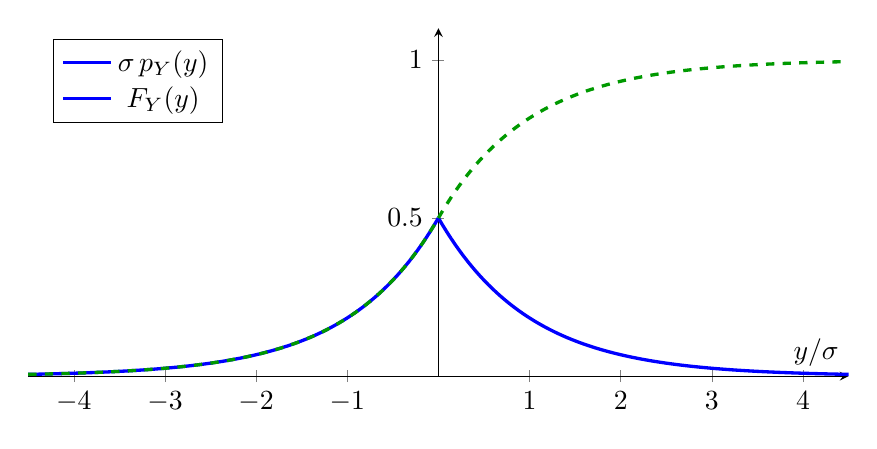
\begin{tikzpicture}
\begin{axis}[
  width=12cm, height=6cm,
  xmin=-4.5, xmax=4.5, ymin=0, ymax=1.1,
  axis lines=center, xlabel={$y/\sigma$}, ylabel={},
  legend pos=north west,
  every axis plot/.append style={very thick},
  samples=100,
]
\addplot[blue, domain=-4.5:0] {0.5*exp(x)};
\addplot[blue, domain=0:4.5] {0.5*exp(-x)};
\addlegendentry{$\sigma\, p_Y(y)$}
\addplot[green!60!black, dashed, domain=-4.5:0] {0.5*exp(x)};
\addplot[green!60!black, dashed, domain=0:4.5] {1 - 0.5*exp(-x)};
\addlegendentry{$F_Y(y)$}
\end{axis}
\end{tikzpicture}
\end{center}

(Dargestellt für $\sigma = 1$; die Dichte ist als $\sigma\, p_Y(y)$ skaliert,
damit sie im selben Maßstab wie $F_Y$ liegt.)

\end{beispiel}

% ---- c) --------------------------------------------------------
\subsubsection*{c) Erwartungswert, zweites Moment, Varianz}

\begin{beispiel}[Momente der Laplace-Verteilung]

\textbf{Gegeben:} $p_Y(y) = \tfrac{1}{2\sigma}\, e^{-|y|/\sigma}$ (zentriert,
$\mu = 0$).

\textbf{Gesucht:} $\mathrm{E}\{Y\}$, $\mathrm{E}\{Y^2\}$, $\mathrm{var}\{Y\}$.

\textbf{Formel} (Momente, Abschnitt~\ref{sec:momente}):

$$
\mathrm{E}\{Y\} = \int_{-\infty}^{\infty} y\, p_Y(y)\,\mathrm{d}y, \qquad
\mathrm{E}\{Y^2\} = \int_{-\infty}^{\infty} y^2\, p_Y(y)\,\mathrm{d}y.
$$

\textbf{Rechnung:}

\emph{Erwartungswert:} Der Integrand $y\, p_Y(y)$ ist ungerade in $y$, die
Dichte symmetrisch um $0$, also

$$
\mathrm{E}\{Y\} = 0.
$$

\emph{Zweites Moment:} Der Integrand $y^2\, p_Y(y)$ ist gerade; mit
$\int_0^{\infty} y^2\, e^{-y/\sigma}\,\mathrm{d}y = 2\sigma^3$ folgt

$$
\mathrm{E}\{Y^2\} = 2 \cdot \frac{1}{2\sigma} \int_0^{\infty} y^2\, e^{-y/\sigma}\,\mathrm{d}y
= \frac{1}{\sigma} \cdot 2\sigma^3 = 2\sigma^2.
$$

\emph{Varianz:}

$$
\mathrm{var}\{Y\} = \mathrm{E}\{Y^2\} - \mathrm{E}\{Y\}^2 = 2\sigma^2 - 0 = 2\sigma^2.
$$

\textbf{Lösung:}

$$
\boxed{\;\mathrm{E}\{Y\} = 0, \qquad \mathrm{E}\{Y^2\} = 2\sigma^2, \qquad
\mathrm{var}\{Y\} = 2\sigma^2\;}
$$

Dies stimmt mit den allgemeinen Werten aus Abschnitt~\ref{sec:laplaceverteilung}
für $\mu = 0$ überein.

\end{beispiel}

% ================================================================
\subsection*{Aufgabe 9.5 – Exponential-Verteilung (Wartezeit)}
% ================================================================

Für ein festes $k = 0$ liefert die Poisson-Verteilung aus Vorrechenaufgabe~9 die
Wahrscheinlichkeit, dass im Beobachtungsintervall der Länge $t = T_B$
\emph{kein} Tropfen fällt:

$$
P\bigl(X(t) = 0\bigr) = e^{-\lambda t}.
$$

Dies ist zugleich die Wahrscheinlichkeit, dass die Wartezeit bis zum ersten
Tropfen größer als $t$ ist. Es gilt $\lambda = 5\,\mathrm{min}^{-1}$.

% ---- a) --------------------------------------------------------
\subsubsection*{a) Kumulative Verteilung der Wartezeit}

\begin{beispiel}[Verteilungsfunktion der Wartezeit]

\textbf{Gegeben:} $P(\text{kein Tropfen bis } t) = P(W > t) = e^{-\lambda t}$ für
$t \geq 0$.

\textbf{Gesucht:} Die kumulative Verteilung $F_W(t) = P(W \leq t)$, also die
Wahrscheinlichkeit, dass innerhalb der Beobachtungszeit $t$ ein Tropfen fällt.

\textbf{Formel} (Gegenereignis):

$$
F_W(t) = P(W \leq t) = 1 - P(W > t)
$$

\textbf{Rechnung:}

$$
F_W(t) = 1 - e^{-\lambda t}, \qquad t \geq 0; \qquad F_W(t) = 0, \quad t < 0.
$$

\textbf{Lösung:}

$$
\boxed{\;F_W(t) = \begin{cases} 1 - e^{-\lambda t} & , \quad t \geq 0 \\[2pt]
0 & , \quad t < 0 \end{cases}\;}
$$

Dies ist die Verteilungsfunktion der Exponentialverteilung
(Abschnitt~\ref{sec:exponentialverteilung}).

\begin{center}
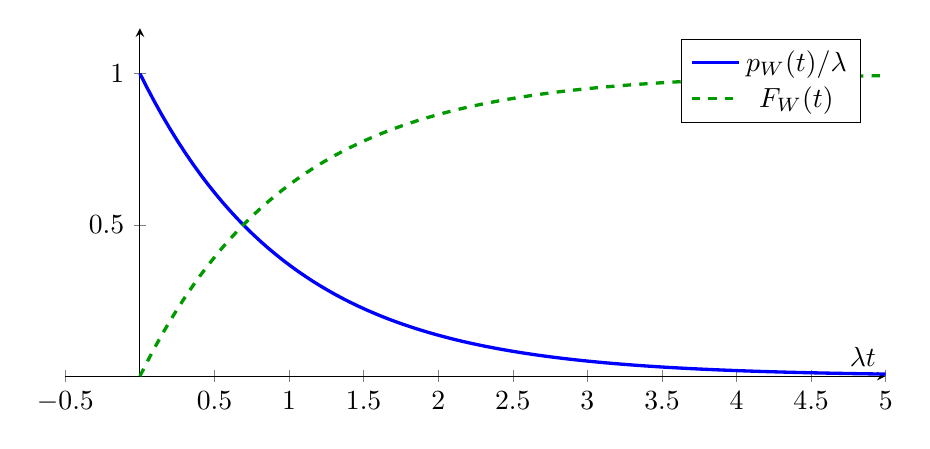
\begin{tikzpicture}
\begin{axis}[
  width=12cm, height=6cm,
  xmin=-0.5, xmax=5, ymin=0, ymax=1.15,
  axis lines=center, xlabel={$\lambda t$}, ylabel={},
  legend pos=north east,
  every axis plot/.append style={very thick},
  samples=100,
]
\addplot[blue, domain=0:5] {exp(-x)};
\addlegendentry{$p_W(t)/\lambda$}
\addplot[green!60!black, dashed, domain=0:5] {1 - exp(-x)};
\addlegendentry{$F_W(t)$}
\end{axis}
\end{tikzpicture}
\end{center}

\end{beispiel}

% ---- b) --------------------------------------------------------
\subsubsection*{b) Wahrscheinlichkeitsdichte der Wartezeit}

\begin{beispiel}[Dichte der Wartezeit durch Ableiten der Verteilungsfunktion]

\textbf{Gegeben:} $F_W(t) = 1 - e^{-\lambda t}$ für $t \geq 0$.

\textbf{Gesucht:} Die Wahrscheinlichkeitsdichte $p_W(t)$.

\textbf{Formel} (Abschnitt~\ref{sec:verteilungsfunktion}):

$$
p_W(t) = \frac{\mathrm{d}}{\mathrm{d}t} F_W(t)
$$

\textbf{Rechnung:}

$$
p_W(t) = \frac{\mathrm{d}}{\mathrm{d}t}\bigl(1 - e^{-\lambda t}\bigr)
= \lambda e^{-\lambda t}, \qquad t \geq 0.
$$

\textbf{Lösung:}

$$
\boxed{\;p_W(t) = \begin{cases} \lambda e^{-\lambda t} & , \quad t \geq 0 \\[2pt]
0 & , \quad t < 0 \end{cases}\;}
$$

Die Wartezeit zwischen zwei Tropfen ist exponentialverteilt mit Parameter
$\lambda$.

\end{beispiel}

% ---- c) --------------------------------------------------------
\subsubsection*{c) Erwartungswert und Varianz der Wartezeit}

\begin{beispiel}[Momente der Exponentialverteilung]

\textbf{Gegeben:} $p_W(t) = \lambda e^{-\lambda t}$ für $t \geq 0$,
$\lambda = 5\,\mathrm{min}^{-1}$.

\textbf{Gesucht:} $\mathrm{E}\{W\}$ und $\mathrm{var}\{W\}$.

\textbf{Formel} (Momente der Exponentialverteilung,
Abschnitt~\ref{sec:exponentialverteilung}):

$$
\mathrm{E}\{W\} = \frac{1}{\lambda}, \qquad \mathrm{var}\{W\} = \frac{1}{\lambda^2}.
$$

\textbf{Rechnung:} Mit $\lambda = 5\,\mathrm{min}^{-1}$:

$$
\mathrm{E}\{W\} = \frac{1}{5}\,\mathrm{min} = 0{,}2\,\mathrm{min} = 12\,\mathrm{s},
\qquad
\mathrm{var}\{W\} = \frac{1}{25}\,\mathrm{min}^2 = 0{,}04\,\mathrm{min}^2.
$$

\textbf{Lösung:}

$$
\boxed{\;\mathrm{E}\{W\} = \frac{1}{\lambda} = 12\,\mathrm{s}, \qquad
\mathrm{var}\{W\} = \frac{1}{\lambda^2} = 0{,}04\,\mathrm{min}^2\;}
$$

Im Mittel vergehen $12\,\mathrm{s}$ zwischen zwei Tropfen -- konsistent mit der
Rate von $5$ Tropfen pro Minute.

\end{beispiel}

% ---- d) --------------------------------------------------------
\subsubsection*{d) Tropfen innerhalb von 10\,s}

\begin{beispiel}[Wahrscheinlichkeit eines Tropfens im Beobachtungsfenster]

\textbf{Gegeben:} Beobachtungsdauer $t = 10\,\mathrm{s} = \tfrac{1}{6}\,\mathrm{min}$,
$\lambda = 5\,\mathrm{min}^{-1}$, also $\lambda t = \tfrac{5}{6}$.

\textbf{Gesucht:} $P(W \leq t)$, dass innerhalb von $10\,\mathrm{s}$ ein Tropfen
fällt.

\textbf{Formel:}

$$
P(W \leq t) = F_W(t) = 1 - e^{-\lambda t}
$$

\textbf{Rechnung:}

$$
P(W \leq 10\,\mathrm{s}) = 1 - e^{-5/6} = 1 - 0{,}4346 = 0{,}5654.
$$

\textbf{Lösung:}

$$
\boxed{\;P(W \leq 10\,\mathrm{s}) = 1 - e^{-5/6} \approx 0{,}5654\;}
$$

Mit rund $56{,}5\,\%$ sieht der Installateur bei einem einzelnen $10$-Sekunden-Blick
einen Tropfen fallen.

\end{beispiel}

% ---- e) --------------------------------------------------------
\subsubsection*{e) $p$-mal 10\,s beobachten -- $q$-mal einen Tropfen sehen}

\begin{beispiel}[Verkettung von Exponential- und Binomialverteilung]

\textbf{Gegeben:} $p$ unabhängige Beobachtungen von je $10\,\mathrm{s}$. In jeder
Einzelbeobachtung wird ein Tropfen mit Wahrscheinlichkeit
$p_1 = 1 - e^{-5/6} = 0{,}5654$ gesehen (aus Teil~d).

\textbf{Gesucht:} Die Wahrscheinlichkeit, in $q$ der $p$ Beobachtungen einen
Tropfen zu sehen.

\textbf{Formel} (Binomialverteilung, Abschnitt~\ref{sec:binomialverteilung}):

$$
P(Q = q) = \binom{p}{q}\, p_1^{\,q}\, (1 - p_1)^{\,p - q}
$$

\textbf{Rechnung:} Da die einzelnen $10$-Sekunden-Beobachtungen unabhängig sind
und jeweils mit Wahrscheinlichkeit $p_1 = 1 - e^{-5/6}$ einen Tropfen liefern
(und mit $1 - p_1 = e^{-5/6}$ keinen), ist die Anzahl $Q$ der erfolgreichen
Beobachtungen binomialverteilt:

$$
P(Q = q) = \binom{p}{q}\, \bigl(1 - e^{-5/6}\bigr)^{q}\,
\bigl(e^{-5/6}\bigr)^{p - q}, \qquad q \in \{0, 1, \dots, p\}.
$$

\textbf{Lösung:}

$$
\boxed{\;P(Q = q) = \binom{p}{q}\, \bigl(1 - e^{-5/6}\bigr)^{q}\,
\bigl(e^{-5/6}\bigr)^{p - q}\;}
$$

Der Erwartungswert der gesehenen Tropfen ist
$\mathrm{E}\{Q\} = p\, p_1 = p\,(1 - e^{-5/6}) \approx 0{,}5654\, p$. Die
kontinuierliche Wartezeitverteilung (Exponential) liefert über
$p_1 = F_W(10\,\mathrm{s})$ die Erfolgswahrscheinlichkeit einer einzelnen
Beobachtung, deren wiederholte Ausführung dann durch die diskrete
Binomialverteilung beschrieben wird.

\end{beispiel}
